\chapter{Cryptographic Security And Known Attacks}
%\chapter{Near-Collision Attack}
 %INTRODUCTION  --> TODO Birthday Attack + General Attack
%TODO 
The main property a hash function must comply to is resitance to collisions (see Section~\ref{sec:requirements}). Therefore, a hashing algorithm is considered to be \emph{broken} if there exists a known attack that enables one to find collisions for the hash function with a time complexity less than a brute force attack.

All the attacks detailed below focus on finding \emph{collisions}. Since resistance to collision attacks implies resistance to pre-image and second pre-image attacks this is the strongest of the cryptographic requirements stated in Section~\ref{sec:requirements}.

We shall hereafter detail what a brute force (also known as Yuval's) attack is, and it's complexity, before exhibiting a few more specific attacks, and their consequences on public confidence in the robustness of algorithms based on the Merkle-Damg\r{a}rd construction.

\section{Brute Force Attack (Yuval's Attack)}
A brute force attack is a trial and error method. A large number of random consecutive guesses are made and the attack is successful if a guess leads to the desired output.

It can be compared to trying many random combinations on a padlock, in which case the attack is successful if the attacker is lucky and tries the correct combination.

Thus, a brute force attack to find collisions for a hash function $H$ will try many random pairs of messages $ (x,x')$ until finding a pair satisfying $x\ne x' $ and $H(x) = H(x')$.

The birthday paradox described bellow provides an estimate of a brute force attack's time complexity, and demonstrates that surprisingly, it doesn't take that many random guesses to get \emph{lucky}. We shall then apply this result to the specific case of finding collisions to hash functions.

\subsection{The Birthday Paradox}
The birthday paradox is a probability argument, referred to as a paradox as it is counter-intuitive.
The idea is that, even though there are 365 days in a year, within a group of 23 or more people the probability of two individuals having the same birthday is higher than $\frac{1}{2}$.

Formally, let us take a group of $k$ individuals, over a period of $n$ days, an let us assume all days are equiprobable as birthdays.
The number of combinations of $k$ different birthdays is $A_n^k=\frac{n!}{n-k!}$. Therefore each individual will have a different birthday with probability $\frac{A_n^k}{n^k}$.

The probability that two people at least will have their birthday on the same day is $$1-\frac{A_n^k}{n^k} \approx 1 - e^{-\frac{k^2}{2 \times n}}$$
This approximation will be justified in Section~\ref{sec:birthday_application}.

Numerically if $k=23$ and $n=365$, the likelyhood two individuals will have their birthday the same day is over 50\%, which is where the name \emph{birthday paradox} comes from. t comes as quite a surprise as we are far from having half as many people as there are days in a year. 
And with a group of 70 people the success probability of this attack increases to 99.9\%!

\subsection{Application To Hashing Functions}~\label{sec:birthday_application}
Let us reformulate the birthday paradox problem, where instead of considering a number of individuals with the same birthday, we consider the number of messages that will have the same digest. This analogy explains why Yuval's attack, which measures a hashing function's resistance to collisions, is dubbed the birthday attack.

We shall denote $H:\mathcal{E} \rightarrow \mathcal{F}$ a hash function chosen randomly from $\mathcal{E}$ to $\mathcal{F}$. Where $\mathcal{E}={\{0,1\}}^*$ and $\mathcal{F}$ is the set of all possible digests output by the hashing algorithm $H$.

Algorithm~\ref{algo:collision} lays out the Yuval attack. The algorithm first creates a set of $k$ messages chosen uniformly and at random from the set of all possible input messages  $\mathcal{E} $. It then tests, for all pairs of messages $(x,x')$, such that $x\ne x'$ within this set, whether they produce the same digest $H(x)=H(x')$.
\begin{algorithm}[H]
\caption{\textsc{Yuval-Find-Collision} (H,k)}
\label{algo:collision}
\begin{algorithmic}[1]
  \State{Randomly choose $\mathcal{M} \subseteq  \mathcal{E} $ such that $\#  \mathcal{M} =k$}
  \ForAll{$x \in  \mathcal{M}$ }
  \State{$y_x \gets H(x)$ }
  \EndFor{}
  \If{$y_x=y_{x'}$ for some $x \ne x'$}
  \Return{$ (x,x') $}
  \Else{}
  \Return{Failure}
  \EndIf{}
 \end{algorithmic}
\end{algorithm}

We whish to estimate $k$, the number of random messages to try, in order to obtain a success probability of finding a collision greater than $\frac{1}{2}$, using Algorithm~\ref{algo:collision}.

In order to measure $H$'s resistance to the Yuval attack, we need to express $k$ as a function of $\#  \mathcal{F} $. In order to do this, let us first evaluate the success probability of Algorithm~\ref{algo:collision}.

We shall denote
\begin{itemize}
  \item $a = \#  \mathcal{F} $.
  \item $P_{Fail}$ the probability that the algorithm finds no collisions.
  \item $P_{Success}=1-P_{Fail}$ the probability that the algorithm finds a collisions.
\end{itemize}

\begin{thm}\label{th:2}
  For any $\mathcal{M}  \subseteq  \mathcal{E}$ such that $\# \mathcal{M} =k$, the success probability of Algorithm~\ref{algo:collision} is $$P_{Success}=1- (\frac{a - 1}{a}) \times (\frac{a - 2}{a}) \times \cdots \times (\frac{a - k + 1}{a}) $$
\end{thm}

\begin{proof}
  In order to prove this theorem, we accept as true that if $H$ is chosen randomly, then $P\lbrack H (x) = y \rbrack = \frac{1}{a}$ for all $x \in  \mathcal{E}$ and all $y \in  \mathcal{F}$.

  Let $\mathcal{M} = \{x_1,x_2,\cdots x_k\}$. And let $E_i$ be the event $''H(x_i) \notin \{H(x_1),h(x_2) \cdots H(x_{i-1})\}''$. Therefore the probability that the algorithm finds no collisions is given by the probability that $\forall i \in \llbracket 1,k \rrbracket$, $E_i$ is true. 

  We have
\begin{equation}
\begin{aligned}
  P\lbrack E_1\rbrack & = 1  \\
  P\lbrack E_i \vert E_1 \wedge E_2 \wedge \cdots \wedge E_{i-1}\rbrack & = \frac{a - i + 1}{a}  \mbox{ for } 2 \le i \le k; \\
  \end{aligned}
\end{equation}

Which gives us:
\begin{equation}
    P_{Fail}=P\lbrack E_1 \wedge E_2 \wedge \cdots \wedge E_{k}\rbrack  = \frac{a -  1}{a} \times \frac{a -  2}{a} \times \cdots \frac{a -  k + 1}{a}
 \end{equation}

    Now we can deduce the probability that the algorithm finds at least one collision:
\begin{equation}
 P_{Success}= 1 - P\lbrack E_1 \wedge E_2 \wedge \cdots \wedge E_{k}\rbrack  \\
\end{equation}
\end{proof}

\vspace{.5cm}

Now that the given theorem has been proven, let us estimate the number of attempts needed to achieve a 50\% chance of finding collisions.
Theorem~\ref{th:2} is equivalent to:
\begin{equation}
P_{Fail}= \prod_{i=1}^{k-1}(1-\frac{i}{a})
\end{equation}
where we can assume $k<<a$, and therefore $\forall i \in \llbracket 1,k \rrbracket$, $\frac{i}{a}<<1$.
Thus we can approximate $1-\frac{i}{a} \approx e^{-\frac{i}{a}}$ which results in:
\begin{equation}
  \begin{aligned}
  P_{Fail} \approx \prod_{i=1}^{k-1}(e^{-\frac{i}{a}}) \\
  P_{Fail} \approx (e^{\sum_{i=1}^{k-1}-\frac{i}{a}}) \\
  P_{Fail} \approx (e^{-\frac{k\times (k-1)}{2*a}}) \\
  \end{aligned}
\end{equation}

Consequently:
\begin{equation}
  P_{Success} \approx 1 - (e^{-\frac{k\times (k-1)}{2*a}}) \\
\end{equation}

For a success probability of $\frac{1}{2}$, this results in:
\begin{equation}
  \begin{aligned}
  0.5 & \approx 1 - (e^{-\frac{k\times (k-1)}{2*a}}) \\
  -\frac{k\times (k-1)}{2*a} & \approx \ln(\frac{1}{2}) \\
  k^2 -k & \approx 2 \times a \times \ln(\frac{1}{2}) \\
  \end{aligned}
\end{equation}

It is logical to assume $k>>1$ since a brute force attack requires many attemps, and therefore $k^2>>k$. In consideration of this, we ignore the term $-k$.

\begin{equation}
  \begin{aligned}
  k & \approx \sqrt{2 \times a \times \ln(\frac{1}{2})} \\
  k & \approx 1.18 \times \sqrt{a}\\
  \end{aligned}
\end{equation}

Hence with just over $\#  \mathcal{F} $ random messages taken in $\mathcal{E}$ the Yuval attack has a fifty-fifty chance of finding a collision for $h$.

\subsection{Complexity Of Renowned Algorithms}
The previous section exposed that the success probability of a brute force attack only depends on the size of the hash function's codomain.

The size of the codomain is a direct result of the digest size: if $\mathcal{F} = {\{ 0,1\}}^n$, $\#  \mathcal{F} = 2^n$.

We can thus easily deduce the complexity of Yuval's attack, executed without any optimisations, against a few renowned hashing algorithms, since the number of attempts in order to reach a fifty percent chance of finding a collision is approximately $1.18 \times 2^{\frac{n}{2}}$.

\begin{itemize}
\item \textbf{MD5} has an output size of 128 bits, the Yuval attack will require just over $2^{64}$ hashes.
  
  With eight NVidia Titan X graphic cards, one can compute 115840 milion md5 hashes per second~\cite{hashcat}
  
 $\frac{2^{64}}{115840 \times 10^6} \approx 1.59 \times 10^8\mbox{ sec } \approx 5 \mbox{ years}$
  
\item \textbf{SHA-1} and \textbf{SHA-0} have an output sizes of 160 bits, the Yuval attack will require over $2^{80}$ hashes.
  
With the previously described setup, this would take $\frac{2^{80}}{115840 \times 10^6}  \approx 330929 \mbox{ years}$

\item The \textbf{SHA-2} and \textbf{SHA-3} families of hash functions have output sizes that vary between 224 bits and 512 bits, and will therefore require $2^{112}$ to $2^{256}$ hash calculations.

  With the previously described setup, for an output of 224 bits, the Yuval attack would take $1.4\times 10^{15}$ years, and an output of 512 bits would take $7.4 \times 10^{48}$ years to reach a success probability of 50\%. 
\end{itemize}

In light of these results, the Yuval attack provides a lower bound to the size of the digest for a hashing algorithm to be secure. In practice a 160-bit (or larger) message digest is recommended.
This is a necessary, but not sufficient, requirement for a cryptographic hash function. Indeed more efficient attacks are possible against hash functions, and when a collision attack is discovered with a lower time complexity than the Yuval attack\footnote{Even if actual collisions have not yet been found.}, the given hash algorithm is said to be \emph{broken}.

Such collision attacks have been discovered against MD5 and SHA-1, and though only theoretical attacks have been published against SHA-1, for MD5, improvements on the brute force attack are such that collisions can be found in seconds!~\cite{Att}.

Though the first great breakthrough in hash cryptanalysis on the Merkle-Damg\r{a}rd construction was acheived by Xiaoyun Wang and al Old in 2004~\cite{WA04}, Marc Stevens published in 2012 a \emph{collision generator} against MD5 which finds collisions within 6 seconds. These attacks rely strongly on a particular type of cryptanalysis called differential cryptanalysis. We shall describe the idea behind differential cryptanalysis in the followig section.


\section{Differential Cryptanalysis Overview}
The most efficient general attacks to date in finding collisions for the MD and SHA family of functions is differential cryptanalysis.

The idea is to construct two \emph{differential paths} which describe precisely the evolution of two input pairs through a given hash function at the same time.

These differential paths examine how differences between two inputs propagate through the compression function's working states. Thus if the desired differential path occurs, one can obtain the desired output difference.
\begin{defn}
A \emph{near-collision attack} is an attack against the compression function, where for two given input values $IHV_{in}$ and $IHV_{in}'$, a differential path is used to find message blocks $M_i$ and $M_i'$ in order to obtain a desired difference in output: $\delta IHV_{out}$.
\end{defn}

The attack takes as input two equal-length sequences of message blocks, called prefixes, $P=M_0,\ldots,M_{i-1}$ and $P'= M'_0,\ldots,M'_{i-1}$ resulting in the same intermediate hash values  $IHV_{i} = IHV'_{i}$. Of course this requirement is easily obtained by choosing these two sequences to be identical, ie $P=P'$. In this case the attack is called an \emph{identical-prefix collision attack} (as opposed to a \emph{chosen-prefix collision attack}).
\begin{defn}
An \emph{identical-prefix collision attack} is a collision attack which finds, given a hash function $H$, and a prefix $P$, two appendages $M \ne M'$ such that $H(P\vert \vert M)=H(P\vert \vert M')$.
\end{defn}
\begin{defn}
A \emph{chosen-prefix collision attack} is a collision attack which finds, given a hash function $H$, and two \emph{different} prefixes $P \ne P'$, two appendages $M \ne M'$ such that $H(P\vert \vert M)=H(P'\vert \vert M')$.   
\end{defn}

In its simplest form, this attack creates two messages $M$ and $M'$ that differ only by two message blocs. These differences will in effect ``compensate'' each other. 

The collision is generated by appending two consecutive pairs of message blocks $(M_i,M_{i+1})$ and $(M'_i,M'_{i+1})$ where $M_i \ne M'_i$ and $M_{i+1} \ne M'_{i+1}$, chosen such that $IHV_{i+2} = IHV'_{i+2}$. Thus all the collision-finding algorithm needs to know is the value of $IHV_{i}$, from which the values of $(M_i,M_{i+1})$ and $(M'_i,M'_{i+1})$ are derived.

The collision attack outputs two messages $M=P\vert \vert M_i \vert \vert M_{i+1}$ and $M'=P\vert \vert M'_i \vert \vert M'_{i+1}$ which result in the same hash.

Due to the incremental nature of the Merkle-Damg\r{a}rd construction, these messages can be extended with identical suffixes, $M=P\vert \vert M_i \vert \vert M_{i+1} \vert \vert S$ and $M'=P\vert \vert M'_i \vert \vert M'_{i+1} \vert \vert S$, and will still produce the same hash.

The general idea behind this attack is depicted in Figure~\ref{fig:collision-attack}.
\vspace{.5cm}

\begin{figure}[!ht]
        \centering
        \begin{tikzpicture}[scale=1.8]

          \draw  [rounded corners, fill=Yellow!10] (-0.3,4) rectangle (9.75,5.2);
          \node [align=center] at (0.5,5){\textbf{Message M}};

          \draw  [rounded corners,fill=Cyan!10] (-0.3,2.8) rectangle (9.75,4);
          \node [align=center] at (0.5,3){\textbf{Message M'}};
        %Box Messages
          \draw  [rounded corners,fill=Green!10] (0,3.5) rectangle (1.7,4.5);
          \node [align=center] at (0.85,4.25){\textbf{Prefix}};
          \node [align=center] at (0.85,3.75){\textbf{$P=M_0,\cdots,M_{i-1}$}};

          \draw  [rounded corners,fill=Green!10] (1.8,3.5) rectangle (3,4.5); \node [align=center] at (2.40,4){\textbf{Padding}};
          
          \draw  [rounded corners,fill=Orange!20] (3.5,4.2) rectangle (5.3,5);
          \node [align=center] at (4.4,4.8){\textbf{near-block}};
          \node [align=center] at (4.4,4.6){\textbf{collision}};
          \node [align=center] at (4.4,4.4){\textbf{$M_i$}};

          \draw  [rounded corners,fill=Purple!20] (3.5,3) rectangle (5.3,3.8);
          \node [align=center] at (4.4,3.6){\textbf{near-block}};
          \node [align=center] at (4.4,3.4){\textbf{collision}};
          \node [align=center] at (4.4,3.2){\textbf{$M'_i$}};

          \draw  [rounded corners,fill=Orange!20] (5.5,4.2) rectangle (7.3,5);
          \node [align=center] at (6.4,4.8){\textbf{near-block}};
          \node [align=center] at (6.4,4.6){\textbf{collision}};
          \node [align=center] at (6.4,4.4){\textbf{$M_{i+1}$}};
          
          \draw  [rounded corners,fill=Purple!20] (5.5,3) rectangle (7.3,3.8);
          \node [align=center] at (6.4,3.6){\textbf{near-block}};
          \node [align=center] at (6.4,3.4){\textbf{collision}};
          \node [align=center] at (6.4,3.2){\textbf{$M'_{i+1}$}};
          
        \draw  [rounded corners,fill=Green!10] (8.25,3.5) rectangle (9.75,4.5);
           \node [align=center] at (9,4){\textbf{Suffix}};
           %Traits et Fleches
         \draw [->, >=latex] (1.7,4) -- (1.8,4);
           
        \draw [->, >=latex] (3,4) -- (3.5,3.4);
        \draw [->, >=latex] (3,4) -- (3.5,4.6);
        
        \draw [->, >=latex] (5.3,3.4) -- (5.5,3.4);
        \draw [->, >=latex] (5.3,4.6) -- (5.5,4.6);
        
        \draw [->, >=latex] (7.3,3.4) -- (8,4);
        \draw [->, >=latex] (7.3,4.6) -- (8,4);

        \node[draw, star, star points=5, star point ratio=.4,fill=Yellow!50]
at (8,4) {\textbf{\textsc{Collision}}};
        \end{tikzpicture}
        \caption{\label{fig:collision-attack}Identical prefix collision attack.}
\end{figure}


\section{Merkle-Damg\r{a}rd Construction Weaknesses}

In addition to the work done on SHA-1 and MD5, which has convinced many cryptographers that these hash functions are no longer secure, the Merkle-Damg\r{a}rd construction itself has severeal inherent weaknesses.
Indeed cryptographic hash functions that rely on this construction are usually assumed to have the three security properties described in Section~\ref{sec:requirements}: collision resistance, preimage resistance, and second preimage resistance. Yet many additional properties are also required of hash functions in practical applications.

Hereafter are a few such requirements that hash functions based on the Merkle-Damg\r{a}rd construction fail to meet:
\begin{itemize}
\item Resistance to \emph{length extension attacks}:
   As demonstrated in Figure~\ref{fig:ExtensionAttack}, due to the incremental structure of the construction, for all $x \in \mathcal{E}$, knowing $H(M_1,M_2,\cdots M_i)$ anyone can calculate  $H(M_1,M_2,\cdots M_i, x)$ without knowing  the values of $M_1,M_2,\cdots M_i$.

  \begin{figure}[ht]
\centering
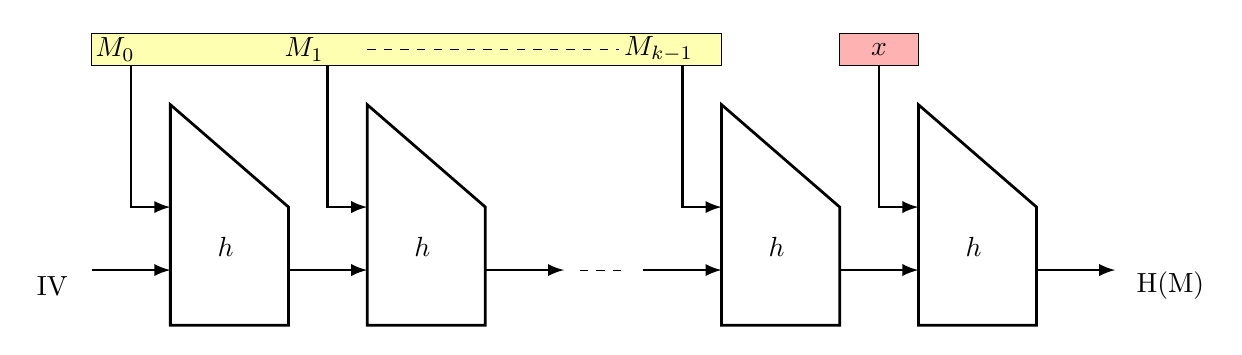
\begin{tikzpicture}

  \draw[fill=Yellow!30] (-1,3.3) rectangle (7,3.7);
  \draw[fill=Red!30] (8.5,3.3) rectangle (9.5,3.7);
\node at (-0.7,3.5){$M_{0}$};
\draw[->, >=latex, line width=1pt] (-0.5,3.3) -- (-0.5,1.5) -- (0,1.5);
\node[align=center] at (-1.5,0.5){IV};
\draw[->, >=latex, line width=1pt] (-1,0.7) -- (0,0.7);
\draw[line width=1pt] (0,0) -- (0,2.8) -- (1.5,1.5) -- (1.5,0) -- cycle;
\node at(0.7,1){$h$};

\node at (1.7,3.5){$M_{1}$};
\draw[->, >=latex, line width=1pt] (2,3.3) -- (2,1.5) -- (2.5,1.5);
\draw[->, >=latex, line width=1pt] (1.5,0.7) -- (2.5,0.7);
\draw[line width=1pt] (2.5,0) -- (2.5,2.8) -- (4,1.5) -- (4,0) -- cycle;
\node at(3.2,1){$h$};
\draw[->, >=latex, line width=1pt] (4,0.7) -- (5,0.7);

\draw[dashed] (5.2,0.7) -- (5.8,0.7);
\draw[dashed] (2.5,3.5) -- (5.7,3.5);

\node at (6.2,3.5){$M_{k-1}$};
\draw[->, >=latex, line width=1pt] (6.5,3.3) -- (6.5,1.5) -- (7,1.5);
\draw[->, >=latex, line width=1pt] (6,0.7) -- (7,0.7);
\draw[line width=1pt] (7,0) -- (7,2.8) -- (8.5,1.5) -- (8.5,0) -- cycle;
\node at(7.7,1){$h$};

\node at (9,3.5){$x$};
\draw[->, >=latex, line width=1pt] (9,3.3) -- (9,1.5) -- (9.5,1.5);
\draw[->, >=latex, line width=1pt] (8.5,0.7) -- (9.5,0.7);
\draw[line width=1pt] (9.5,0) -- (9.5,2.8) -- (11,1.5) -- (11,0) -- cycle;
\node at(10.2,1){$h$};
\draw[->, >=latex, line width=1pt] (11,0.7) -- (12,0.7);
\node[align=center] at (12.7,0.5){H(M)};

\end{tikzpicture}
\caption{\label{fig:ExtensionAttack}Extension attack against the Merkle-Damg\r{a}rd construction.}
\end{figure}

\item Resistance to \emph{multi-collision attacks}:
  \begin{defn}Given a hash function H, a \emph{ multi-collision or r-multi-collision attack} finds many messages with the same hash value, ie: $r$ messages $\{ M^{(1)} \cdots M^{(r)}\}$,  such that $H(M^{(1)} )= H(M^{(2)})= \cdots H(M^{(r)})$.
  \end{defn}
  It has been proven by Antoine Joux~\cite{MC04} that finding multicollisions on iterated hash functions based on the Merkle-Damg\r{a}rd construction is not much harder than finding ordinary collisions.

\item Resistance to \emph{herding attacks}~\cite{HH06}:
  \begin{defn} In a \emph{herding attack}, the adversary first commits to a hash value and is then provided with a prefix. The attacker is required to find a suitable suffix that “herds” to the previously committed hash value. That is, given $x$, $h$, and a hash function $H$, the adversary must find $y$ such that $H(x\vert \vert y)=h$.

    A hash function that resists to herding attacks is said to be \emph{Chosen Target Forced Prefix (CTFP) preimage resistant}.
  \end{defn}
\end{itemize}

\vspace{.5cm}

 These vulnerabilities of the Merkle-Damg\r{a}rd construction emphasize the opinion that the next generation of hashing algortithms to be standardised and widely deployed must rely on a fundamentally new underlying structure. 
